% Chapter 1

\chapter{Introduction} % Main chapter title

\label{Chapter1} % For referencing the chapter elsewhere, use \ref{Chapter1} 

%----------------------------------------------------------------------------------------

% Define some commands to keep the formatting separated from the content 
\newcommand{\keyword}[1]{\textbf{#1}}
\newcommand{\tabhead}[1]{\textbf{#1}}
\newcommand{\code}[1]{\texttt{#1}}
\newcommand{\file}[1]{\texttt{\bfseries#1}}
\newcommand{\option}[1]{\texttt{\itshape#1}}






%1----------------------------------------------------------------------------------------



\section{Contexte}



Le déclin massif de la glace arctique ces dernières décennies est considéré comme l'une des manifestations les plus marquantes du réchauffement climatique \parencite{stroeve2012trends}. Ce déclin présente des enjeux aussi climatiques qu'industriels. Premièrement, grâce à son étendue et son épaisseur immense, la zone arctique est un contributeur majeur au climat à travers ses échanges de chaleurs par rayonnement avec l'atmosphère. Il est donc crucial de considérer l'évolution de la glace de mer dans les modèles climatiques. Deuxièmement, la chute de cette couverture de glace dans la MIZ\footnote{Marginal Ice Zone : zone de transition entre l’océan et le c\oe{}ur de la banquise, où la concentration de glace est inférieure à $80$\%, et/ou les morceaux de glace sont de faible épaisseur ($\approx 1 \text{m}$) et de petite taille ($10 \text{m} - 100 \text{km}$).} (voir \cref{fig:miz}) ouvre des routes maritimes facilitant l'exploitation de ses réserves d’hydrocarbures (qui, à ce jour, restent quasiment intactes). Il est donc important dans ce contexte de pouvoir prédire l'évolution de la banquise dans l'Arctique (au moins) à court terme.


Parmi les éléments exacerbant ce déclin de la glace dans l'Arctique, des études ont cité l'accélération de la vitesse et de la déformation des floes\footnote{Un floe est un morceau individuel de glace rencontré dans la MIZ.} \parencite{rampal2011ipcc,spreen2011trends}. Pour les prédictions de l'évolution de la banquise, les modèles qui considèrent l'étendu de glace comme un milieu continu ne sont pas adaptés, surtout à l'échelle de la MIZ. Au contraire, les modèle granulaires, bien que plus coûteux, doivent être privilégiés afin de prendre en compte la nature discontinue de la banquise ainsi que sa rhéologie\footnote{Étude de la résistance des matériaux aux contraintes et aux déformations.}. Des modèles granulaires pour l'évolution de la glace ont été utilisés par le passé \parencite{hopkins1996mesoscale,kjerstad2014modeling}. Cependant, les approches utilisées dans ces travaux limitent la géométrie (circulaire, rectangulaire) et le nombre de floes (de l'ordre de la centaine) et modélisent le contact entre floes comme une répulsion après interpénétration\footnote{Les détails sur le contact avec interpénétration sont donnés dans la \cref{sec:thesematthias}.} (voir \parencite[p.16]{balasoiu2020halthesis}). 

En 2015, M. Rabatel, S. Labbé et J. Weiss \parencite{rabatel2015dynamics,rabatel2015thesis} ont développé un nouveau modèle granulaire prenant en compte la collision des floes sans passer par un processus d’interpénétration (voir \cref{fig:simugranu1}). Dans leur modèle, le mouvement des floes vérifie les équations de préservation du moment angulaire et de la quantité de mouvement. Le modèle prend en compte la force de Coriolis et les interactions avec l’océan et l’atmosphère. En 2020, D. Balasoiu \parencite{balasoiu2020halthesis} développe un modèle de fracture dans le but de le coupler au modèle granulaire d'interaction préexistant, en prenant en compte le phénomène de percussion\footnote{Dans ce rapport, nous désignerons par \emph{percussion} la série de collisions à très courts intervalles de temps entre deux ou plusieurs floes.}. Les floes de glace auparavant considérés comme des corps solides dans les travaux de M. Rabatel, sont dorénavant élastiques. En plus de proposer un modèle de fracture fragile pour les floes de glace, D. Balasoiu obtient l’expression du déplacement limite d'un floe (considéré comme un réseau de masses reliées par des ressorts à fortes raideurs) qui est percuté par un objet ponctuel.

C'est dans ce contexte que le projet \href{https://sasip-climate.github.io/}{SASIP} a été lancé. Il s'agit d'un projet dont le but est de développer un nouveau modèle de glace de mer capable d'appréhender sa dynamique complexe afin d'améliorer sa représentation dans les futurs modèles de prédiction climatique. Cette gigantesque entreprise, pilotée par l'Institut des Géosciences de l'Environnement regroupe dix partenaires internationaux parmi lesquels la France, la Norvège, les Etats-Unis d'Amérique, l'Italie, le Royaume-Unis et l'Allemagne. Ce fut un grand honneur pour moi d'intégrer ce projet dans un stage de six mois avec pour missions de prendre en main et de poursuivre le développement du modèle de fracturation des floes existant ; puis d'intégrer ce modèle dans un code de calcul de l’évolution de la banquise à l’échelle des floes de glace.


\begin{figure}[!h]
    \centering
    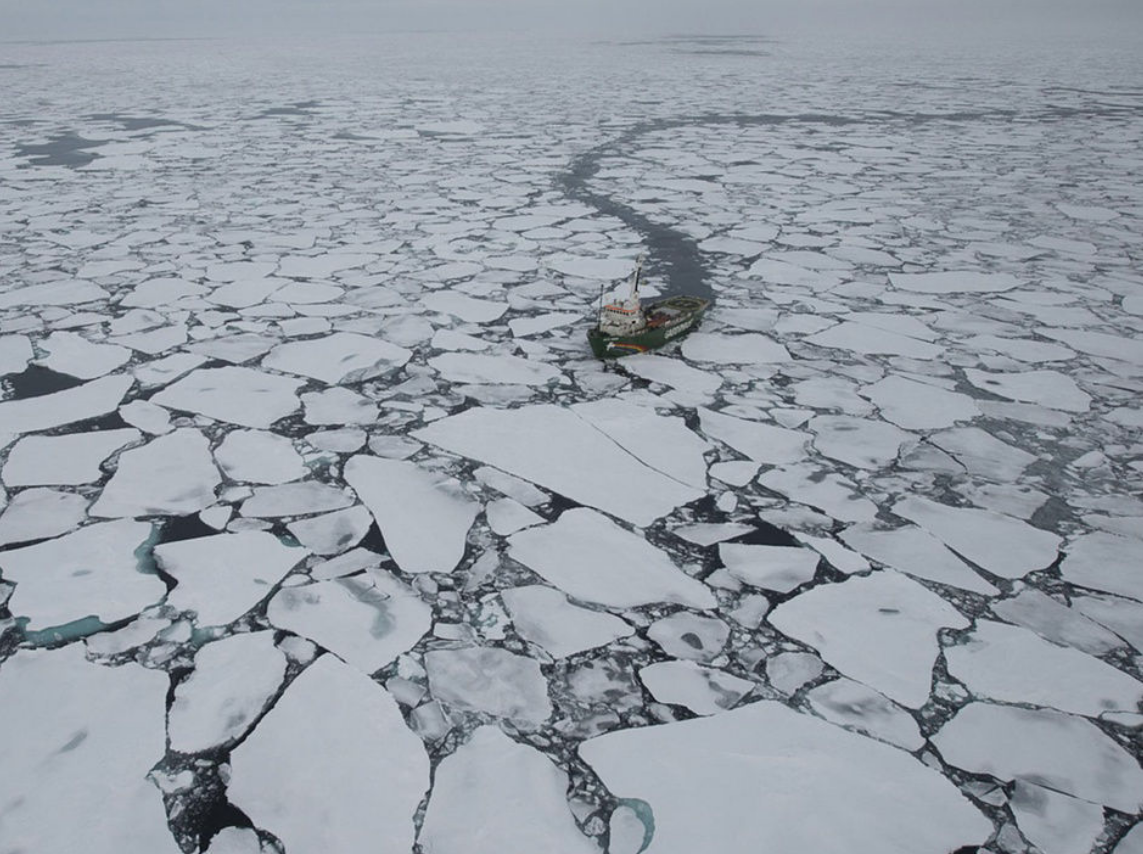
\includegraphics[width=0.55\textwidth]{IceRoutes.png}
    \caption{Un bateau industriel dans la MIZ.}
    \label{fig:miz}
\end{figure}

\begin{figure}[!h]
    \centering
    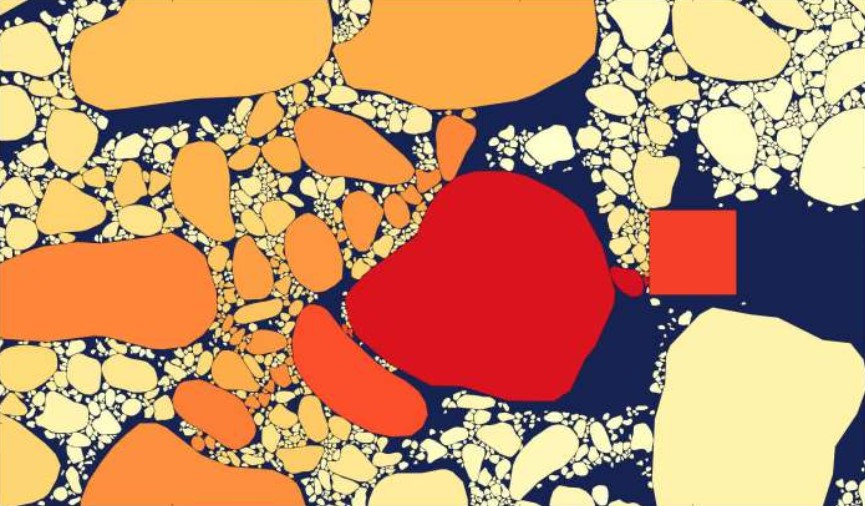
\includegraphics[width=0.65\textwidth]{SimuGranu1.jpg}
    \caption{Capture d’écran d’une simulation d’interaction glace structure avec contact rigide \parencite[p.23]{balasoiu2020halthesis}.}
    \label{fig:simugranu1}
\end{figure}


%2----------------------------------------------------------------------------------------





\section{Problématique}


Ce stage a été pour moi une opportunité qui m'a amené à explorer la percussion et la fracture des floes de glace. J'ai eu à développer un modèle mathématique et à l'intégrer à un projet de développement logiciel. Plus précisément, ce rapport de stage se développe au prisme de la problématique du comportement d'un matériau élastique lors de la percussion avec un matériau voisin. En utilisant les principes de mécanique du contact et les équations différentielles, nous nous sommes intéressés à la question : \emph{Comment le matériau se déplace-t-il après de tel(s) choc(s)?} Nous nous sommes aussi posés la question de savoir \emph{dans quelle mesure une fracture apparait-elle dans le matériau ?} Pour cette dernière tâche, nous nous sommes basés sur le modèle de Griffith et sur l'approche variationnelle de Francfort-Marigot.






%3----------------------------------------------------------------------------------------





\section{Environnement}


Mon stage s'est déroulé du \DTMdisplaydate{2021}{02}{03}{-1} au \DTMdisplaydate{2021}{07}{31}{-1} au sein du \href{https://www.ljll.math.upmc.fr/en/?lang=fr}{Laboratoire Jacques-Louis Lions} (LJLL) de Sorbonne Université, sous la supervision du Professeur Stéphane Labbé. Ce stage s'inscrit dans la continuation directe de deux thèses effectuée par Matthias Rabatel \Parencite{rabatel2015thesis} et Dimitri Balasoiu \parencite{balasoiu2020halthesis} au sein du \href{https://www-ljk.imag.fr/}{Laboratoire Jean Kuntzmann} de l'Université Grenoble Alpes, codirigée par le Professeur Stéphane Labbé et Monsieur Jérôme Weiss, en collaboration avec le groupe TOTAL. Le LJLL a constitué un environnement idéal pour ce travail de stage de par ses membres spécialisés dans divers domaines des mathématiques appliquées, et des ressources mises à ma disposition pour mener à bien mes fonctions. Cependant, malgré la convivialité et l'esprit d'équipe régnant au sein de ce laboratoire, j'ai dû effectuer certaines tâches en télétravail ; ceci principalement dû à la situation de confinement imposée en France durant cette période trouble de pandémie de COVID-19.



%4----------------------------------------------------------------------------------------





\section{Objectifs}
\label{sec:introobk}

Au vu des problèmes qui nous sont donnés de résoudre et des travaux qui ont précédé, nos \textbf{objectifs primaires} pour ce rapport de stage (ainsi que leur temps approximatif d'exécution) sont les suivants :
\begin{enumerate}
    \item Comprendre le modèle de rupture de Griffith dans les milieux élastiques en s'appropriant les travaux précédents \emph{(6 semaines)} ;
    \item Comprendre le passage micro/macro du modèle élastique pour travailler sur le modèle de percussion \emph{(20 semaines)} ; 
    \item Intégrer le modèle dans un code de calcul de l’évolution
    de la banquise à l’échelle des floes de glace \emph{(0 semaines)}.
\end{enumerate}

\noindent Afin de remplir au mieux ces missions, nous les avons séparées en groupes de tâches singulières formant ainsi des \textbf{objectifs secondaires} étalés sur six mois (26 semaines) que sont:   

\begin{itemize}
    \item Prise en main de la notion de $\Gamma$-convergence en calcul des variations ;
    \item Lecture et assimilation de la thèse de Matthias Rabatel \parencite{rabatel2015thesis} ;
    \item Lecture et assimilation de la thèse de Dimitri Balasoiu \parencite{balasoiu2020halthesis} ;
    \item Modéliser, simuler et visualiser le déplacement d'un floe en une dimension (1D) après une collision ;
    \item Modéliser, simuler et visualiser le déplacement d'un floe en deux dimensions (2D) après une collision ;
    \item Implémenter le modèle de fracture de Griffith dans le modèle de collision 1D préexistant.
\end{itemize}



En vue de rendre compte de manière fidèle et analytique des six mois passés au sein du Laboratoire Jacques-Louis Lions, il apparaît logique de présenter à titre préalable les remarquables travaux qui ont précédés ce stage (\cref{Chapter2}); puis de présenter les différents modèles de glace de mer développés et étudiés en 1D (\cref{Chapter3}) ; ensuite en 2D (\cref{Chapter4}). Enfin, à l'aide d'un journal de bord, il sera précisé les différentes tâches que nous avons pu effectuer, et les nombreux apports que j'en ai tiré (\cref{Chapter5}). 





%5----------------------------------------------------------------------------------------




\section{Abstract}


The rapid shrinking of the Arctic ice cap these last decades is seen as one of the most striking manifestations of global warming \parencite{stroeve2012trends}. This decrease in size opens way to new opportunities, namely the creation of routes beneficial to the industrial sector. The second major consequence of this observation that we need to include the Marginal Ice Zone (MIZ) into climate prediction models. In 2015, Rabatel et al. \parencite{rabatel2015dynamics,rabatel2015thesis} developed a sophisticated model for the dynamics of rigid ice floes. The model was later enhanced by Balasoiu in 2020 when he considered the ice floe not as rigid, but as an elastic material modeled by a mass-spring-damper lattice \parencite{balasoiu2020halthesis}. Our main goal in this report is to study what happens when two or more ice floes collide (percussion, fracture, etc.), both in 1D and in 2D.
